\chapter{Solution Design}
\label{sec:solution}

    % •	What is the physical structure of cotton candy?
    % What aspects define “quality” of cotton candy?     •	What are the key factors that affect quality?
    % •	How does it change with production parameters?
    % What we already learned doing cc is -> The notes from the notion

\section{Design Goals and Approach}
% High-level aims (why a prescriptive DT, bottom-up design, reproducibility).
The overarching goal of this work is to design a prescriptive digital twin that can monitor, predict, and actively recommend process adjustments in real time. Unlike purely predictive twins, the prescriptive variant enables actionable feedback loops, improving product quality under changing environmental conditions. The system follows a bottom-up design philosophy, relying on real-world sensor data, edge computing, and physical experimentation rather than top-down simulations. This approach ensures that the twin reflects the actual behavior of the system, including variability and noise inherent to physical processes. Moreover, the architecture emphasizes reproducibility and modularity: all components are based on accessible hardware and lightweight services, allowing for future adaptation to similar manufacturing or experimental setups.


\section{System Architecture}
% Conceptual block diagram: sensors, machine, twin, data collection.

The experimental setup is based on a commercial cotton candy machine (Model RCZK-1030-W, Royal Catering~\cite{ccmachine-manual}), which features two physical controls: a main power switch and a separate heating element switch. The robot interacting with the machine is a Universal Robots UR5e robotic arm equipped with a 2F-85 adaptive gripper~\cite{ur5e-manual}.

The robot executes a series of predefined tasks throughout the cotton candy production process. These include: activating the machine and heating elements, opening a food-grade funnel to dispense sugar into a spoon, inserting the spoon content into the machine head, selecting a wooden stick, positioning it at the center of the rotating head, and performing controlled circular and vertical movements to collect the cotton candy. After spinning, the robot transfers the completed cotton candy into a storage case and then powers down the heating and turns off the machine.

Each step is facilitated by custom-designed 3D-printed components, which support the precise positioning and secure handling of tools and materials. These include holders for the funnel, the wooden sticks, the final product, and grip enhancements for the spoon. All CAD models are available online~\cite{cc-cad-models}.

\begin{figure}[h]
    \centering
    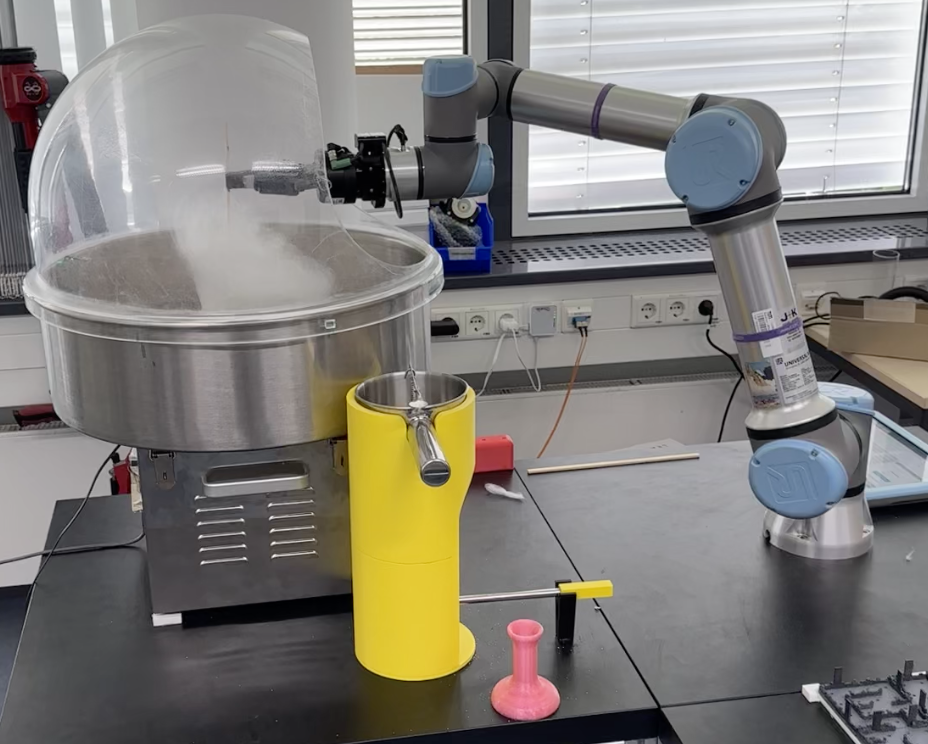
\includegraphics[width=0.85\linewidth]{figures/creating_cc.png}
    \caption{Machine and Robot Arm working together to create Cotton Candy.}
    \label{fig:creating_cc}
\end{figure}

The robot's task sequences are orchestrated using \textbf{CPEE} (Cloud Process Execution Engine)~\cite{mangler2022cloudprocessexecutionengine}, a lightweight service-based workflow engine designed for executing and monitoring process models. Each robotic action—such as filling the spoon or positioning the stick is modeled as a service node in a CPEE process. These workflows are triggered and monitored via HTTP interfaces, allowing for modular, distributed execution logic and easy integration with the digital twin infrastructure.

%-Probably put this in the Implementation
We attempted to adjust the speed of the robot arm dynamically via the REST API, but the internal safety mechanisms of the UR5e controller automatically downscaled the speed since it exceeded feasible limits. For example, when we doubled the target speed, the controller reduced the speed scaling factor to 0.5, effectively cancelling the change. As a result, parameterizing interaction speed—despite being a potential quality-impacting variable—had to be excluded from the implementation. Prior research has indicated that robot speed and motion control can influence product quality in Cotton Candy production~\cite{TERASHIMA2022139953}.


\section{Sensor Design and Placement}
\subsection{Temperature Sensors}
% Infrared + ambient.
To capture the thermal dynamics of the cotton candy production process, we employed both ambient and infrared temperature sensors. These measurements are essential for monitoring the heating behavior of the machine head and understanding how temperature influences product formation.

\paragraph{Infrared Object Temperature Sensor}
To monitor the thermal behavior of the cotton candy machine's rotating head, we use a non-contact infrared temperature sensor (MLX90614). This sensor is well suited for the application due to its high accuracy (±0.5°C in the critical 0–50°C range) and wide measurement span, covering object temperatures from --70°C up to 380°C. These properties make it ideal for tracking the heating phase where the sugar melts and begins to form cotton candy.

Although only one sensor is used during regular operation, we conducted a dedicated experiment using a second sensor to evaluate placement and correlation. One sensor was positioned inside the machine, 3cm above the rotating head, while the other was mounted below the machine base, pointing sideways toward the head at the same distance. Over 2000 seconds, both sensors recorded temperature data to assess the relationship between internal and external readings.

\begin{figure}[h]
    \centering
    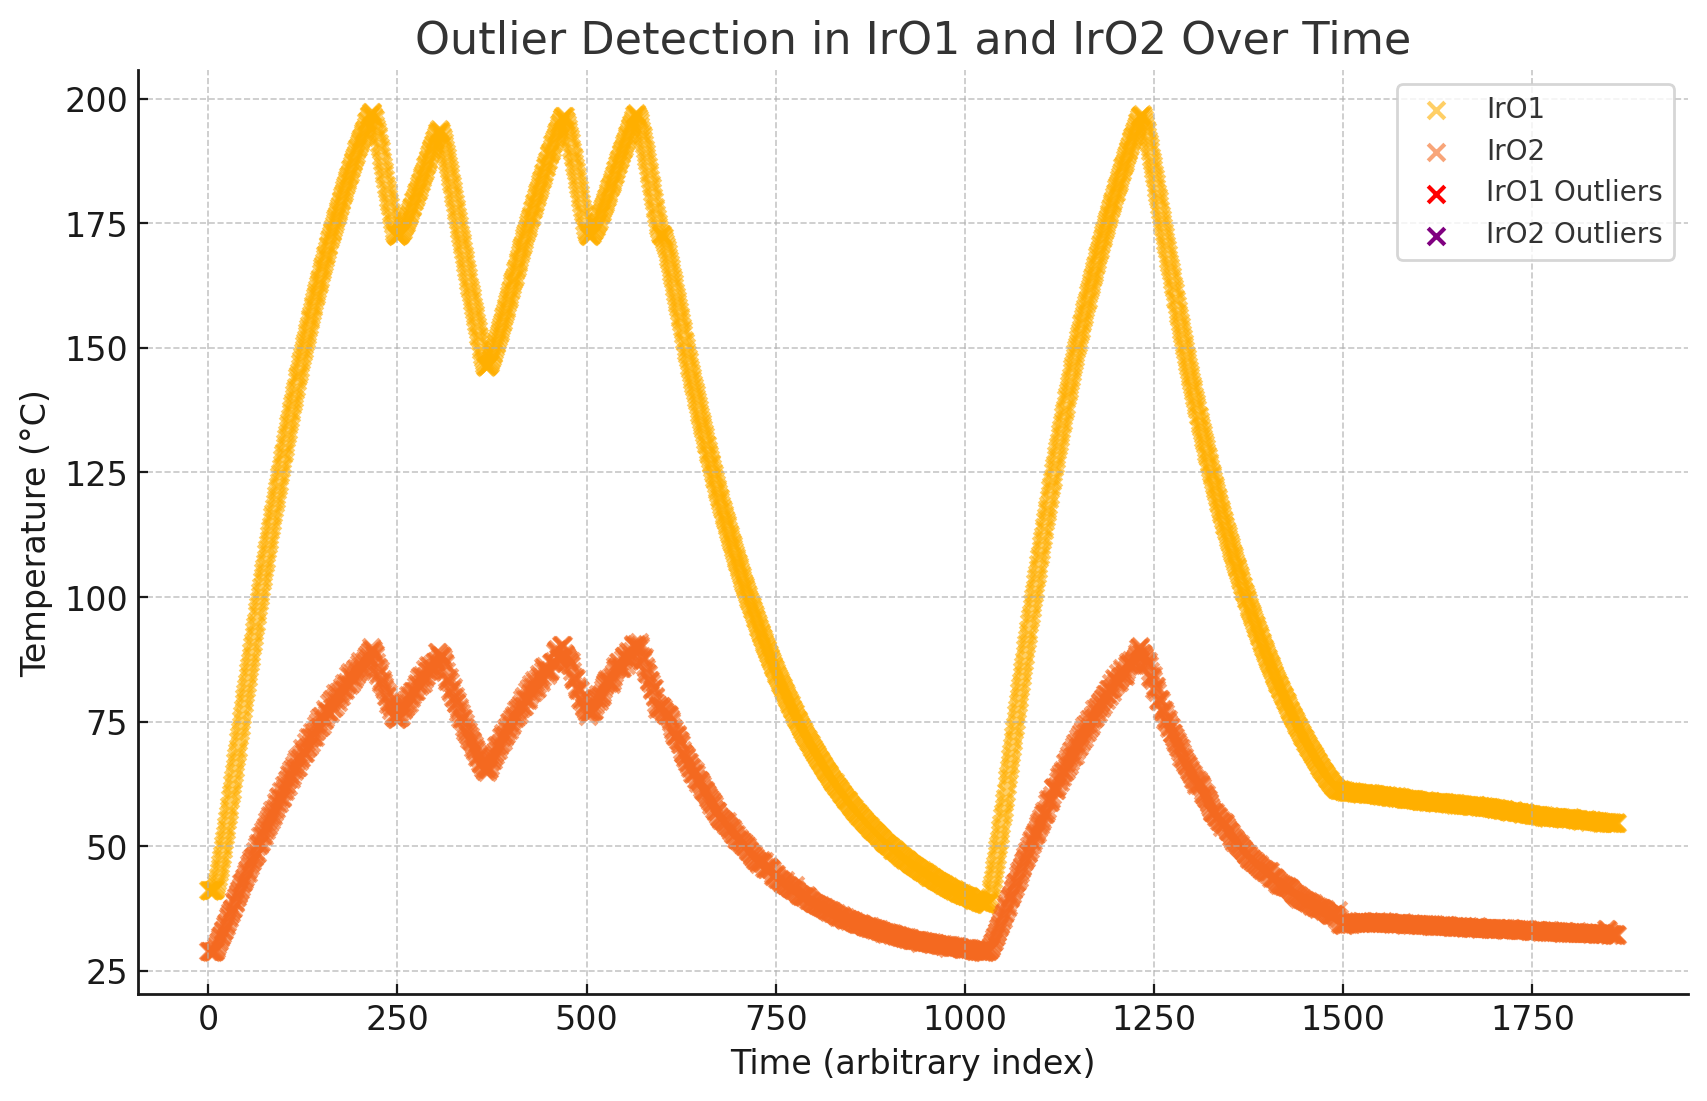
\includegraphics[width=0.85\linewidth]{figures/IrO1 and IrO2 Over Time.png}
    \caption{Comparison of internal (IrO1) and external (IrO2) infrared temperature sensors over 2000 seconds.}
    \label{fig:ir-comparison}
\end{figure}

A linear regression analysis showed a strong correlation between the two sensors, with a coefficient of determination $R^2 = 0.996$, slope $a = 0.383$, and intercept $b = 12.15$. The resulting model for estimating the external temperature $T_{\text{outside}}$ based on the internal reading $T_{\text{inside}}$ is:

\[
T_{\text{outside}} = 0.383 \cdot T_{\text{inside}} + 12.15
\]

This strong correlation implies that the internal head temperature can be reliably estimated from the external measurement. Consequently, the system design employs only a single infrared temperature sensor mounted outside the head during operation. This placement avoids obstructing the cotton candy formation process while maintaining accurate and reliable thermal monitoring. The sensor’s communication protocol and technical specifications are described in the official documentation~\cite{waveshareIRsensor}.

\subsection{Humidity Sensors}
% Inside vs outside, offset explanation.
To monitor moisture conditions during cotton candy production, we used high-precision HDC3021 temperature and humidity sensors, featuring a typical relative humidity accuracy of ±1.5\%. One sensor is positioned outside the machine to measure ambient conditions, while the other is placed inside the enclosure to capture internal humidity near the process area. Given that small variations in ambient humidity can significantly affect fiber formation, stickiness, and shrinkage, this level of precision—combined with dual placement—is essential for capturing process-relevant environmental dynamics within the digital twin.

\subsection{Humidity Sensor Offset}
During idle phases, the inside humidity sensor consistently showed 2--5\% higher values than the outside reference. This effect is best explained by placement and airflow, since it disappeared once the machine was running. Replacing the sensors produced the same pattern, confirming it is not sensor wear but an environmental effect. For the digital twin, this means that differences observed during operation can be interpreted as true process dynamics, such as moisture accumulation, rather than calibration bias.

\subsection{Energy Monitoring}
% Plug sensor and rationale.
To track the energy consumption of each production cycle, we integrated a smart plug (Delock 11827) between the cotton candy machine and its power source. This device measures real-time power usage and cumulative energy per process, providing valuable insights into operational efficiency and enabling energy-aware optimization within the digital twin.

\section{Cotton Candy Product Characteristics}
% \subsection{What we learned empirically doing CC}
%     - write times, forms, radius why that radius etc etc etc
%     => We can create a formula of how we think it behaves, that we can compare afterwards in the Data Recollection Evaluation.
% \subsection{Physical Structure}
% % Amorphous vs crystalline, thermal study.

% \subsection{Quality Indicators}
% % Volume density, compression test, etc.
% \paragraph{How to measure quality indicatros} A scale -> model -> connected via a service.

% \subsection{Excluded Factors}
% % Taste, visual appearance, long-term hygroscopic behavior.

Cotton candy is composed primarily of spun sucrose, which can exist in amorphous or crystalline form depending on production and environmental conditions. As prior thermal studies have shown, higher humidity tends to promote crystallization, which affects the product's texture, stability, and shelf-life~\cite{TERASHIMA2022139953}. In our empirical work, we observed that structural properties such as volume, density, and compression resistance varied depending on production parameters like humidity level, cooking time, and airflow. While visual appearance, texture, and taste are relevant to perceived quality, we excluded them due to their subjective nature or the complexity of capturing them reproducibly. Instead, we focused on measurable indicators: volume density (grams per known volume), weight and compression resistance, which serve as practical proxies for structural characteristics. These properties are recorded using a connected scientific scale and a simple model that integrates with the digital twin via service calls.


\section{Process Parameters and Environmental Factors}
% \subsection{Humidity}
% % Effects during spinning and after; airflow.

% \subsection{Temperature}
% % Limited control, cooking time as proxy.

% \subsection{Spinning Speed}
% % Fixed.

% \subsection{Sugar Amount and Formulation}
% % Fixed, supermarket sugar.

Several environmental and process parameters are expected to influence cotton candy quality. Humidity, in particular, plays a critical role in fiber formation and post-spinning stability, with higher relative humidity leading to stickier and denser products. Temperature is less directly controllable in our setup, but the duration of heating and spinning acts as a practical proxy. Other variables, such as spinning speed and sugar formulation, remain fixed due to hardware constraints and reproducibility concerns. Based on these considerations, the prescriptive digital twin is designed to map measurable environmental conditions and controllable process parameters to observable quality outcomes.

\section{Prescriptive Digital Twin Design}
% How environment + process map to quality.
% Forecasting with decision trees.
% High-level evaluation plan.
The goal of the prescriptive digital twin is not only to model the cotton candy production process but also to recommend process adjustments that improve product quality under varying environmental conditions. The twin receives input from real-time environmental sensors (e.g., humidity and ambient temperature) and selected process parameters such as cooking time and sugar amount. Quality is evaluated through measurable indicators like volume and compression resistance, which serve as outcome variables. To map input conditions to these outcomes, we employ decision tree models, chosen for their interpretability, low training complexity, and ability to capture non-linear decision boundaries in small datasets. The prescriptive layer is designed to traverse these decision trees in reverse, identifying optimal process configurations under given environmental constraints. While the modeling and evaluation are carried out in the implementation phase, this design defines the structure and logic of the prescriptive system.


% \section{    •	What is the physical structure of cotton candy?}
% Cotton candy is primarily composed of spun sucrose, which can exist in two main forms:WHat we saw in the paper\dots

% \section{What aspects?}

% YES: Volume density -> How much sugar is in a given volume -> Weighing sample and measuring volume (water displacement) => Doing this wiht a trichter that has the exact volume written. How does it change wiht more or less humidity?

% NO: Visual appearance -> Fiber structure, color, consistency -> Visual inspection, photography + image analysis (even with your phone and Python/OpenCV) => we are not gonna do this because we learned that it is not really possible to distinguish the fibers with the naked eye. Its a full master thesis on its own

% NO: Texture \& mouthfeel -> Stickiness, softness, “melt-in-mouth” -> Manual touch test, break force => Stickiness is interesting to measure but probably difficult more on it later 
% NO: Hygroscopic behavior -> Stickiness as it absorbs moisture -> Weighing sample over time at room humidity => This is very interesting, takes time to measure but hey -> NO BC WE WILL CREATE THEM IN DIFF ENVIRONMENTS AND CANNOT CREATE A CONTROL CAPSULE

% YES: Crispness vs softness -> Related to crystallinity -> Compression test (kitchen scale or small force sensor) => It would mean measureing how much compression force is needed to break the fibers, very difficult, we build a model that we could test between CC and after measuring volume we weighted it, we tested this and that and concluded\dots

%  B. Compression Test
% 	•	Use a small kitchen scale or force sensor.
% 	•	Press gently until collapse starts.
% 	•	Record maximum weight/force applied.
% 	•	Amorphous cotton candy tends to be softer; more crystalline samples resist compression.
% % ➡ Proxy for structure & texture.

% NO: Structural stability -> How long it holds shape over time -> Timed visual check at room conditions => Takes long to test, 

% NO: Taste (subjective) -> Flavor preception is too subjective so we will not do this, but it is important to note that it is a factor in quality perception.

% \section{    •	How does it change with production parameters?}
% How can we change the environment and control so that production parameters are changed 
%     •	Humidity: Higher humidity leads to more stickiness and faster recrystallization. -> How to simulate Humidity?
%     The gas environment during spinning directly changes how much of the sucrose becomes crystalline vs amorphous.
% 	•	More oxygen \& moisture → more crystallization.
% 	•	Less oxygen \& low moisture (like nitrogen or dry air) → more amorphous content.
%     -> We cannot change the environment, but we can change the humidity of the process with:
%         - Airflow / fans -> Stronger air movement near spinner -> Helps dry fibers during flight/creation, reduces moisture pickup.
%     -> YESSSS LETS DO THIS

%     % IMPORTANt
%     Affect on more humidity durign spinning -> Fibers may break sooner, become shorter, thicker. fibers stick together more.
%     and after spinning -> Fibers collapse and shrink, Loss of volume (shrinkage), stickiness increases. what about compression?
%     Immediately after spinning (fresh)
% - Fibers in humid air are thicker, stickier → denser structure → higher compression resistance initially (less fluffy, more “compact”). - Less air trapped between fibers → more force needed to compress.
% Shortly after spinning (as moisture is absorbed)
% - As fibers absorb moisture, they soften → compression force quickly drops. - Structure collapses under small loads.
% % IMPORTANt

% Compression is kind of complicated to test since: 
% Actually, at high humidity:
% 	•	At first → more compact = higher compression resistance.
% 	•	But as time passes → absorbs moisture → weaker structure = lower compression resistance.

% In contrast, at low humidity:
% 	•	The fibers stay dry, fluffy, and light.
% 	•	Lower compression resistance but much better structural stability over time.

%     Humidity Level
%         Result that we think we could achieve:
%         Low RH \(<30\%\)
%         Light, fluffy, large volume, fine fibers.
%         High RH \(>60\%\)
%         Denser, smaller volume, coarser fibers, faster shrinkage.


%     •	Temperature: Higher temperatures can lead to more amorphous structure, but too high can cause burning. We have no control over this, as we are gonna see in the Solution Design, we are using a machine that always stays at the same ratio of temperature when at work. 
%     -> What we can control and change is the Cooking time, so the temperature that the head had when inserting the suagr and the time that we let the cotton candy get created, and let the arm roll. -> What this hopefully gives us is the change in structure that we can test with the compression test and a bigger volume.

%     •	Spinning speed: Faster spinning may lead to finer fibers, affecting texture. Spinning speed (Higher RPM) Creates finer fibers, helps counteract thickening effect of humidity. -> We cannot control this. The given machine always spins in the same speed.

%     -  One big variable that I had at the start was the Sugar amount. Thinking naively, I thought that more sugar would lead to more volume, but this is not the case. The amount of sugar in the process is always the same, and we are not changing it. We are always using the same amount of sugar for each production, which is 10 grams. -> Adding more won’t help volume, might increase stickiness. And we are not measuring this change in stickiness as we saw before.

%     - Sugar formulation -> Use anti-hygroscopic additives (e.g., small \% of maltodextrin or stabilizers) -> Slows moisture absorption. Often used in industrial production. We are not chanign the sugar formulation. We are always using the same sugar from the supermarket for making it easier to reproduce the results.



% \section{Prescriptive Digital Twin Flow}

% - We have an Environment that we cannot control, but we can measure it.
% - We have a process that we can control, but what exactly? THe time of cook? (Yes) The amunt of sugar? (Yes, but doesnt impact), The heating up before spinning? (Yes, but only energy savings impact) The \dots
% - We have a product that we can measure and evaluate the quality, but how? (First measure the Volume and then the compression stress, etc) 

% With 200 points of this data we can create a Model that can forecast the quality mark of the product looking at the ENV and the Process Rules. With Desicion Trees since this and that\dots

% With the Forecasting we can change the Process rules to imporve the quality of the product. How? With Decision Trees? Trasvering back? How should it be done? I dont know yet.


% \begin{figure}[h]
%     \centering
%     \caption{My Figure Caption}
%     
\includegraphics[width=0.7\textwidth]{tum-resources/images/Universitaet_Flaggen.jpg}
%     \floatfoot{A note describing the figure}
%     \label{fig:firstFigure}
% \end{figure}




% %Maybe Trash
% \section{Thermal Study on Cotton Candy}
% Cotton candy consists of spun sucrose that cools rapidly, forming a mostly amorphous structure — but:
% 	•	Over time, this amorphous state can convert into crystalline form.
% 	•	The ratio between crystalline and amorphous sucrose affects:
% 	•	Texture
% 	•	Stability
% 	•	Taste
% 	•	Shelf-life

% % The paper investigates how the physical structure of cotton candy changes depending on how it is produced and stored, focusing especially on how much is amorphous vs crystalline sucrose.
% % 	•	The author studies this using Differential Scanning Calorimetry (DSC), a thermal analysis technique to measure transitions like glass transitions, crystallization, and melting.
% % 	•	The novelty: the study compares cotton candy spun in air vs in nitrogen atmosphere to see how different gas environments affect its physical and thermal properties.

% % In essence, it’s a study of the physics of sugar in cotton candy — very relevant to your Cotton Candy Automata project, as this kind of data gives insight into the material side of your digital twin.

% This paper provides very solid experimental data on how production parameters influence the physical structure (crystalline vs amorphous) of cotton candy.

% Crystalline is \dots
% Amorphous is \dots

% % Because the amorphous vs crystalline ratio affects:
% % 	•	Shelf life (amorphous recrystallizes over time)
% % 	•	Stability (stickiness, collapse, hardening)
% % 	•	Thermal behavior (different melting/glass transition points)
% % 	•	Quality (texture, mouthfeel)

% Knowing how production parameters (like gas environment) affect structure can inform optimal production recipes. We are not gonna compare CCA vs CCN, since we are always using Normal Air but
% We learn about the importance of humidity, and want to use it for our Data Recollection since this is important For the Prescriptive twin design.

% This helps with us taking the decision how to measure the quality of CC when doing data recollection and giving a note to the process.

% What makes it difficult is that the changes are fine and little, and we dont really know if we are gonna be able to distinguish them, but we did research and will introducte this in the Solution Design.


